\documentclass[dvipsnames]{beamer}
\usepackage[utf8]{inputenc}
\usepackage{listings}
\usepackage{comment}
\usepackage{soul}
%\usepackage{ulem}
\usepackage{subfig}
\setul{}{1pt}
\usepackage[oldenum, olditem]{paralist}
%allow even smaller text
\newcommand\tinytiny{\fontsize{4pt}{3}\selectfont}

\makeatletter
\let\old@lstKV@SwitchCases\lstKV@SwitchCases
\def\lstKV@SwitchCases#1#2#3{}
\makeatother
\usepackage{lstlinebgrd}
\makeatletter
\let\lstKV@SwitchCases\old@lstKV@SwitchCases

\lst@Key{numbers}{none}{%
    \def\lst@PlaceNumber{\lst@linebgrd}%
    \lstKV@SwitchCases{#1}%
    {none:\\%
     left:\def\lst@PlaceNumber{\llap{\normalfont
                \lst@numberstyle{\thelstnumber}\kern\lst@numbersep}\lst@linebgrd}\\%
     right:\def\lst@PlaceNumber{\rlap{\normalfont
                \kern\linewidth \kern\lst@numbersep
                \lst@numberstyle{\thelstnumber}}\lst@linebgrd}%
    }{\PackageError{Listings}{Numbers #1 unknown}\@ehc}}
\makeatother


\graphicspath{{logos/}}

\usepackage{tikz}
\graphicspath{{3_6/figures/}}
%disclaimer for Sandia. uncomment and the whole blob goes away @ b80c116300122
\def\sandid{SAND2020-7755 PE}

% \title{Performance Portability with Kokkos}
\title{Kokkos 3.6 Release Briefing}

%BAD misuse of author field
\author{New Capabilities}


\usetheme{kokkos}

\newif\ifshort
\newif\ifmedium
\newif\iffull
\newif\ifnotoverview

\newcommand{\TutorialDirectory}{\texttt{Intro-Full}}
\newcommand{\ExerciseDirectory}[1]{\texttt{Exercises/#1/}}
\newcommand{\TutorialClone}{\texttt{Kokkos/kokkos-tutorials/\TutorialDirectory}}

\definecolor{darkgreen}{rgb}{0.0, 0.5, 0.0}
\definecolor{darkred}{rgb}{0.8, 0.0, 0.0}
\definecolor{orange}{rgb}{0.8, 0.33, 0.0}
\definecolor{purple}{rgb}{0.60, 0.20, 0.80}
\colorlet{bodyColor}{blue!20}
\colorlet{patternColor}{orange!30}
\colorlet{policyColor}{green!30}

% http://tex.stackexchange.com/questions/144448/color-a-text-line-in-a-code-lstlisting
\lstnewenvironment{code}[1][]%
{
  %with txfonts: OT1/txr/m/n/10
  %with default fonts: OT1/cmr/m/n/10
  %\fontfamily{cmr}\selectfont
  %\showthe\font
   \noindent
   \minipage{\linewidth}
   %\vspace{0.5\baselineskip}
   \lstset{mathescape, escapeinside={<@}{@>},
moredelim=**[is][{\btHL[fill=patternColor]}]{@pattern}{@pattern},
moredelim=**[is][{\btHL[fill=red!30]}]{@warning}{@warning},
moredelim=**[is][{\btHL[fill=policyColor]}]{@policy}{@policy},
moredelim=**[is][{\btHL[fill=bodyColor]}]{@body}{@body},
moredelim=**[is][{\btHL[fill=red!30]}]{@warning}{@warning},
moredelim=**[is][\color{black}]{@black}{@black},
moredelim=**[is][\color{blue}]{@blue}{@blue},
moredelim=**[is][\bf]{@bold}{@bold},
moredelim=**[is][\it]{@italic}{@italic},
moredelim=**[is][\color{boldblue}\bf]{@boldblue}{@boldblue},
moredelim=**[is][\color{red}]{@red}{@red},
moredelim=**[is][\color{green}]{@green}{@green},
moredelim=**[is][\color{gray}]{@gray}{@gray},
moredelim=**[is][\color{darkgreen}]{@darkgreen}{@darkgreen},
moredelim=**[is][\color{darkred}]{@darkred}{@darkred},
moredelim=**[is][\color{orange}]{@orange}{@orange},
moredelim=**[is][\color{purple}]{@purple}{@purple},
keywords={},
#1}
}
{
  \endminipage
  %\vspace{1.0\baselineskip}
}

\makeatletter
\newif\ifATOlinebackground
\lst@Key{linebackground}{\tiny}{\def\ATOlinebackground{#1}\global\ATOlinebackgroundtrue}
\makeatother

\lstnewenvironment{shell}[1][]{%
  \global\ATOlinebackgroundfalse
  \lstset{language=sh,%
    showstringspaces=false,
    aboveskip=0pt,
    frame=none,
    numbers=none,
    belowskip=2pt,
    breaklines=true,
    #1,
    }
  %\ifATOlinebackground
  \lstset{linebackgroundcolor={
    \ATOlinebackground
  }}
  %\fi
  }{}

\lstnewenvironment{cmake}[1][]{%
  \global\ATOlinebackgroundfalse
  \lstset{language=sh,%
    showstringspaces=false,
    aboveskip=0pt,
    frame=none,
    numbers=none,
    belowskip=2pt,
    breaklines=true,
    #1,
    }
  %\ifATOlinebackground
  \lstset{linebackgroundcolor={
    \ATOlinebackground
  }}
  %\fi
  }{}

\newcommand{\inlinecode}[1]{{\lstset{basicstyle=\ttfamily,keywordstyle={},showstringspaces=false}\lstinline$#1$}}
\newcommand{\inlineshell}[1]{{\lstset{basicstyle=\ttfamily,keywordstyle={},showstringspaces=false}\lstinline$#1$}}

\setbeamercolor{block title}{fg=white, bg=SandiaLightBlue}
\setbeamercolor{block body}{bg=lightgray}
\setbeamercolor{block title alerted}{fg=white, bg=SandiaRed}
\setbeamercolor{block body alerted}{bg=lightgray}



%\usepackage[texcoord,grid,gridunit=mm,gridcolor=red!10,subgridcolor=green!10]{eso-pic}
\usepackage[absolute,overlay]{textpos}





% http://tex.stackexchange.com/questions/8851/how-can-i-highlight-some-lines-from-source-code

\usepackage{pgf, pgffor}
\usepackage{listings}
\usepackage{lstlinebgrd} % see http://www.ctan.org/pkg/lstaddons

\makeatletter
%%%%%%%%%%%%%%%%%%%%%%%%%%%%%%%%%%%%%%%%%%%%%%%%%%%%%%%%%%%%%%%%%%%%%%%%%%%%%%
%
% \btIfInRange{number}{range list}{TRUE}{FALSE}
%
% Test in int number <number> is element of a (comma separated) list of ranges
% (such as: {1,3-5,7,10-12,14}) and processes <TRUE> or <FALSE> respectively

\newcount\bt@rangea
\newcount\bt@rangeb

\newcommand\btIfInRange[2]{%
    \global\let\bt@inrange\@secondoftwo%
    \edef\bt@rangelist{#2}%
    \foreach \range in \bt@rangelist {%
        \afterassignment\bt@getrangeb%
        \bt@rangea=0\range\relax%
        \pgfmathtruncatemacro\result{ ( #1 >= \bt@rangea) && (#1 <= \bt@rangeb) }%
        \ifnum\result=1\relax%
            \breakforeach%
            \global\let\bt@inrange\@firstoftwo%
        \fi%
    }%
    \bt@inrange%
}
\newcommand\bt@getrangeb{%
    \@ifnextchar\relax%
        {\bt@rangeb=\bt@rangea}%
        {\@getrangeb}%
}
\def\@getrangeb-#1\relax{%
    \ifx\relax#1\relax%
        \bt@rangeb=100000%   \maxdimen is too large for pgfmath
    \else%
        \bt@rangeb=#1\relax%
    \fi%
}

%%%%%%%%%%%%%%%%%%%%%%%%%%%%%%%%%%%%%%%%%%%%%%%%%%%%%%%%%%%%%%%%%%%%%%%%%%%%%%
%
% \btLstHL<overlay spec>{range list}
%
% TODO BUG: \btLstHL commands can not yet be accumulated if more than one overlay spec match.
%
\newcommand<>{\btLstHL}[2]{%
  \only#3{\btIfInRange{\value{lstnumber}}{#1}{\color{#2}\def\lst@linebgrdcmd{\color@block}}{\def\lst@linebgrdcmd####1####2####3{}}}%
}%
\makeatother






% http://tex.stackexchange.com/questions/15237/highlight-text-in-code-listing-while-also-keeping-syntax-highlighting
%\usepackage[T1]{fontenc}
%\usepackage{listings,xcolor,beramono}
\usepackage{tikz}

\makeatletter
\newenvironment{btHighlight}[1][]
{\begingroup\tikzset{bt@Highlight@par/.style={#1}}\begin{lrbox}{\@tempboxa}}
{\end{lrbox}\bt@HL@box[bt@Highlight@par]{\@tempboxa}\endgroup}

\newcommand\btHL[1][]{%
  \begin{btHighlight}[#1]\bgroup\aftergroup\bt@HL@endenv%
}
\def\bt@HL@endenv{%
  \end{btHighlight}%
  \egroup
}
\newcommand{\bt@HL@box}[2][]{%
  \tikz[#1]{%
    \pgfpathrectangle{\pgfpoint{1pt}{0pt}}{\pgfpoint{\wd #2}{\ht #2}}%
    \pgfusepath{use as bounding box}%
    \node[anchor=base west, fill=orange!30,outer sep=0pt,inner xsep=1pt, inner ysep=0pt, rounded corners=3pt, minimum height=\ht\strutbox+1pt,#1]{\raisebox{1pt}{\strut}\strut\usebox{#2}};
  }%
}
\makeatother



\usetikzlibrary{calc}
\usepackage{xparse}%  For \NewDocumentCommand

% tikzmark command, for shading over items
\newcommand{\tikzmark}[1]{\tikz[overlay,remember picture] \node (#1) {};}

\makeatletter
\NewDocumentCommand{\DrawBox}{s O{}}{%
    \tikz[overlay,remember picture]{
    \IfBooleanTF{#1}{%
        \coordinate (RightPoint) at ($(left |- right)+(\linewidth-\labelsep-\labelwidth,0.0)$);
    }{%
        \coordinate (RightPoint) at (right.east);
    }%
    \draw[red,#2]
      ($(left)+(-0.2em,0.9em)$) rectangle
      ($(RightPoint)+(0.2em,-0.3em)$);}
}

\NewDocumentCommand{\DrawBoxWide}{s O{}}{%
    \tikz[overlay,remember picture]{
    \IfBooleanTF{#1}{%
        \coordinate (RightPoint) at ($(left |- right)+(\linewidth-\labelsep-\labelwidth,0.0)$);
    }{%
        \coordinate (RightPoint) at (right.east);
    }%
    \draw[red,#2]
      ($(left)+(-\labelwidth,0.9em)$) rectangle
      ($(RightPoint)+(0.2em,-0.3em)$);}
}

\NewDocumentCommand{\DrawBoxWideBlack}{s O{}}{%
    \tikz[overlay,remember picture]{
    \IfBooleanTF{#1}{%
        \coordinate (RightPoint) at ($(left |- right)+(\linewidth-\labelsep-\labelwidth,0.0)$);
    }{%
        \coordinate (RightPoint) at (right.east);
    }%
    \draw[black,#2]
      ($(left)+(-\labelwidth,0.9em)$) rectangle
      ($(RightPoint)+(0.2em,-0.3em)$);}
}
\makeatother

\usetikzlibrary{positioning}

\usetikzlibrary{shapes}

\hypersetup{
    colorlinks=true,
    linkcolor=blue,
    filecolor=magenta,
    urlcolor=cyan,
}



\shorttrue
\mediumfalse
\fullfalse

\begin{document}

\begin{frame}
	\titlepage
\end{frame}


\begin{frame}[fragile]{Outline}

\textbf{3.6 Release Higlights}

\begin{itemize}
   \item{Kokkos Core}
   \begin{itemize}
     \item{CMake Language Build Support}
     \item{UniqueToken Improvements}	     
     \item{More View Allocation Properties Support}
     \item{C++ Standard Algorithms}
     \item{Math Traits}
   \end{itemize}
   \item{KokkosKernels}
\end{itemize}

\end{frame}

\begin{frame}{Find More}

\textbf{Online Resources}:

\begin{itemize}
        \item \url{https://github.com/kokkos}:
                \begin{itemize}
                        \item Primary Kokkos GitHub Organization
                \end{itemize}
        \item \url{https://github.com/kokkos/kokkos-tutorials/wiki/Kokkos-Lecture-Series}:
                \begin{itemize}
			\item{Slides, recording and Q\&A for the Full Lectures}
                \end{itemize}
        \item \url{https://github.com/kokkos/kokkos/wiki}:
                \begin{itemize}
                        \item Wiki including API reference
                \end{itemize}
        \item \url{https://kokkosteam.slack.com}:
                \begin{itemize}
                        \item Slack channel for Kokkos.
                        \item Please join: fastest way to get your questions answered.
                        \item Can whitelist domains, or invite individual people.
                \end{itemize}
\end{itemize}

\end{frame}


%==========================================================================

\begin{frame}[fragile]{}

  {\Huge CMake Build Language}

  \vspace{10pt}

  \textbf{Content:}
  \begin{itemize}
    \item {Using CMakes Language Extension Support}
    \item {CUDA for Windows}
  \end{itemize}

  \vspace{-20pt}

\end{frame}

%==========================================================================

\begin{frame}[fragile]{What is CMake Language Support}
   Every source file CMake compiles has a \textit{language}

   \begin{itemize}
     \item {Default == file extension (.cpp, .c, .f90, ...)}
     \item {But you can set it: \texttt{set\_source\_files\_properties(f.bar PROPERTIES LANGUAGE CXX)}}
   \end{itemize}

   \textbf{Why does this matter for Kokkos?}

   \vspace{10pt}
   CMake treats some language extensions that way, but not all:
   
   \begin{itemize}
     \item {CUDA $->$ CMake language \texttt{CUDA}}
     \item {HIP $->$ CMake language \texttt{HIP}}
     \item {OpenMP $->$ \textbf{Not} a CMake language.}
     \item {SYCL $->$ \textbf{Not} a CMake language.}
   \end{itemize}
\end{frame}

\begin{frame}[fragile]{Kokkos and CMake Language}

  \textbf{Pre 3.6 behavior}

  \begin{itemize}
    \item {All Kokkos containing files are C++ files (CXX)}
    \item {Kokkos's build system adds compiler flags to make files CUDA, HIP, OpenMP, or SYCL}
    \begin{itemize}
      \item {We add \texttt{-fopenmp, -x cu, ...}}
    \end{itemize}
    \item {We use \texttt{nvcc\_wrapper} to make CMake not choke on \texttt{nvcc}}
  \end{itemize}

  \textbf{Advantages:}
  \begin{itemize}
    \item {Flags can be obtained via depending on target, language \texttt{NOT}}
    \item {Support for HIP before CMake supported it}
    \item {No need for users to set the correct language for each file - \textit{Note:} the \textit{need} propagates, the setting doesn't ...}
  \end{itemize}

  \textbf{Drawbacks:}
  \begin{itemize}
    \item {Not fully using CMakes native CUDA and HIP support}
    \item {\texttt{nvcc\_wrapper} only works on Linux}
  \end{itemize}

	
\end{frame}


\begin{frame}[fragile]{Kokkos and CMake Language}

  \textbf{3.6 behavior}

  
  \begin{itemize}
    \item {Default: same as pre 3.6}
    \item {Set \texttt{-DKokkos\_ENABLE\_COMPILE\_AS\_CMAKE\_LANGUAGE=ON} to use CMake Language mode.}
    \item {Use \texttt{set\_source\_files\_properties} on each source file depending on Kokkos}
    \begin{itemize}
      \item{We export \texttt{Kokkos\_COMPILE\_LANGUAGE} to make that portable}
    \end{itemize}
  \end{itemize}

  \textbf{Pifalls:}
  \begin{itemize}
    \item {\texttt{CMAKE\_CXX\_FLAGS} unused by Kokkos files}
    \begin{itemize} 
      \item{\texttt{CMAKE\_CUDA\_FLAGS} for CUDA (equiv. for HIP)}
      \item{\texttt{CMAKE\_CXX\_FLAGS} for SYCL/OpenMP etc.}
    \end{itemize}
    \item{YOU need to set \texttt{CMAKE\_CUDA\_ARCHITECTURES} downstream}
    \item{YOU need to add \texttt{Kokkos\_COMPILE\_LANGUAGE} to your project!}
    \item{For libraries: your users need to set all this too ..}
    \item{Interaction with MPI Wrappers iffy ...}
  \end{itemize}


\end{frame}

\begin{frame}[fragile]{CMake Language Example}
\textbf{Configure Kokkos:}
\begin{lstlisting}[language=bash]
cmake -DKokkos_ENABLE_CUDA=ON -DKokkos_ARCH_VOLTA70=ON \
  -DKokkos_ENABLE_COMPILE_AS_CMAKE_LANGUAGE=ON ${KOKKOS_SOURCE}
\end{lstlisting}

\textbf{Project CMakeLists.txt:}
\begin{lstlisting}[language=bash]
#find Kokkos before project declaration
find_package(Kokkos COMPONENTS separable_compilation)

project(Example CXX Fortran ${Kokkos_COMPILE_LANGUAGE})

set_source_files_properties(cmake_example.cpp PROPERTIES 
  LANGUAGE \${Kokkos_COMPILER_LANGUAGE})

add_executable(example cmake_example.cpp bar.cpp foo.f)

target_link_libraries(example Kokkos::kokkos)
\end{lstlisting}

\textbf{Configure Project:}

\begin{lstlisting}[language=bash]
cmake -DCMAKE_CUDA_ARCHITECTURES=70 ${PROJECT_SOURCE}
\end{lstlisting}

\end{frame}

\begin{frame}[fragile]{When Should One Use This?}
\textbf{Why should I use this, with all the complication?}
\begin{itemize}
  \item{You may want to use native CMake CUDA/HIP support}
  \item{You may hate \texttt{nvcc\_wrapper}}
  \item{But most importantly:}
\end{itemize}

\begin{center}
\textbf{This works in Visual Studio for MSVC + NVCC!}
\end{center}

\end{frame}
%==========================================================================
%


%==========================================================================

\begin{frame}[fragile]

        {\Huge Deprecated in release 3.6}

  \vspace{-20pt}

\end{frame}

%==========================================================================

\begin{frame}[fragile]{Deprecated}

Configure with \texttt{-DKokkos\_ENABLE\_DEPRECATED\_CODE\_3=OFF} to disable   

\begin{itemize}
\item Array reductions with pointer return types
\item \texttt{OpenMP::\{validate\_partition,partition\_master\}}
\item \texttt{KOKKOS\_ACTIVE\_EXECUTION\_MEMORY\_SPACE\_*} macros and \texttt{ActiveExecutionMemorySpace} alias
\item \texttt{log2(unsigned) -> int}
\end{itemize}

\end{frame}

\begin{frame}[fragile]{Namespace Change}
\begin{center}
Not technically deprecation since it was in non-backward guaranteeing state!
\end{center}
\texttt{Kokkos::Impl::} $->$ \texttt{Kokkos::}
\begin{code}	
    is_array_layout
    is_execution_policy
    is_execution_space
    is_memory_space
    is_memory_traits
    is_space
    is_view
    SpaceAccessibility
    Timer  // also header impl/Kokkos_Timer.hpp
\end{code}


\texttt{Kokkos::Experimental::} $->$ \texttt{Kokkos::}
\begin{code}
    Iterate
    MDRangePolicy
    Rank
\end{code}
\end{frame}


\begin{frame}[fragile]{Removed}

Removed:

\begin{code}
    KOKKOS_ACTIVE_EXECUTION_MEMORY_SPACE_HOST/DEVICE
    Kokkos::Impl::ActiveExecutionMemorySpace
    Kokkos::Impl::verify_space
    Kokkos::Experimental::MasterLock
    OpenMP/HPX::partition_master
    int log2(int) // we got double log2(INTEGRAL) and REAL log2(REAL)
\end{code}

\texttt{is\_space} member types removed:
\begin{code}
    is_space::host_memory_space
    is_space::host_execution_space
    is_space::host_mirror_space
\end{code}
\end{frame}


\begin{frame}[fragile]{Backend Specific Things}

CUDA and HIP Error management functionality removed, which should never have been public:
\begin{code}
    CudaSpace::access_error()
    CudaUVMSpace::number_of_allocations()
    CUDA_SAFE_CALL
    HIPSpace::access_error()
    HIP_SAFE_CALL
\end{code}

Only partially supported by backends:
\begin{code}
    TeamPolicy::vector_length() // only existed for some backends
\end{code}

Behavior change in \texttt{UnorderedMap}:
\begin{code}
    UnorderdMap::value_at(i) with i>=capacity()
    UnorderdMap::key_at(i) with i>=capacity()
\end{code}
\end{frame}


\begin{frame}[fragile]{Interface Changes and Configure}
Change in argument order:
\begin{code}
    // deprecated
    create_mirror_view(space, view, WithoutInitializing);
    // new
    create_mirror_view(WithoutInitializing, space, view);
\end{code}

Array reductions:
\begin{itemize}
  \item Array reductions, have a runtime length array as result.
  \item Only supported with functors, not lambdas (one has to define \texttt{value\_type} and \texttt{value\_count} as members)
  \item Deprecated the option to provide raw pointer as the result argument for \texttt{parallel\_reduce}, use a \texttt{View} instead.
\end{itemize}

Configure options Removed:
\begin{code}
	Kokkos_ARCH_EPYC -> ZEN/ZEN2 depending on platform
	Kokkos_ARCH_RYZEN -> ZEN/ZEN2 depending on platform
	Kokkos_ARCH=
	Kokkos_DEVICES=
\end{code}
\end{frame}


%==========================================================================

\begin{frame}[fragile]{}

  {\Huge Threads is now std::threads}

  \vspace{10pt}

  \textbf{Content:}
  \begin{itemize}
    \item {Configure Changes}
  \end{itemize}

  \vspace{-20pt}

\end{frame}

%==========================================================================

\begin{frame}[fragile]{std::thread instead of pthread}
   We are now using std::thread instead of raw pthread
  \begin{itemize}
    \item {No code change necessary - implementation detail of Kokkos}
    \item {Makes the \texttt{Kokkos::Threads} backend work on Windows}
    \item {The backend is more interoperable with other C++ facilities}
  \end{itemize}

  One change: can't use \texttt{Kokkos\_ENABLE\_PTHREADS} as CMake option.
  \begin{itemize}
    \item \texttt{Kokkos\_ENABLE\_THREADS} is the new option
    \item We still export \texttt{Kokkos\_ENABLE\_PTHREAD} for downstream users.
  \end{itemize}
\end{frame}

\begin{frame}[fragile]{}

  {\Huge Improved \texttt{UniqueToken}}

  \vspace{10pt}

  \textbf{Content:}
  \begin{itemize}
    \item {Configure Changes}
  \end{itemize}

  \vspace{-20pt}

\end{frame}

\begin{frame}[fragile]{UniqueToken Recap}
\textbf{What is UniqueToken}

\vspace{3pt}
\texttt{UniqueToken} is a portable way to acquire a unique ID for the calling thread.

\begin{itemize}
  \item{ID is within a given range}
  \item{Can be used similar to a \textit{thread-id}}
  \item{Most commonly used to acquire a resource from a resource-pool}
  \begin{itemize}
    \item{E.g. per-thread temporary memory buffer}
    \item{Used internally for random generator pool}
  \end{itemize}
\end{itemize}

   \begin{code}[frame=single, keywords={UniqueToken,size,acquire,release}]
    UniqueToken<ExecutionSpace> token;
    int number_of_uniqe_ids = token.size();
    RandomGenPool pool(number_of_unique_ids,seed);
    parallel_for("L", N, KOKKOS_LAMBDA(int i) {
      int id = token.acquire();
      RandomGen gen = pool(id);
      ...
      token.release(id);
    });
   \end{code}

\end{frame}

\begin{frame}[fragile]{Performance Improvement}
\textbf{Identified Massive Performance Bug}

\begin{code}[frame=single, keywords={UniqueToken,size,acquire,release,atomic_add,memory_fence}]
 UniqueToken<ExecutionSpace> token;
 int N = token.size(); int M = N*x;
 View<double**> dest(N,R), src(M,R);

 parallel_for("UT", M, KOKKOS_LAMBDA(int i) {
   int j = token.acquire(); memory_fence();
   for(int k=0; k<R; k++) dest(j,k) += src(i,k);
   memory_fence(); token.release(j);
 });

 parallel_for("A" M, KOKKOS_LAMBDA(int i) {
   for(int k=0; k<R; k++) atomic_add(&dest(j,k), src(i,k));
 });
\end{code}

\end{frame}

\begin{frame}[fragile]{Performance Improvement}
\textbf{Identified Massive Performance Bug}

\vspace{3pt}

\begin{center}
  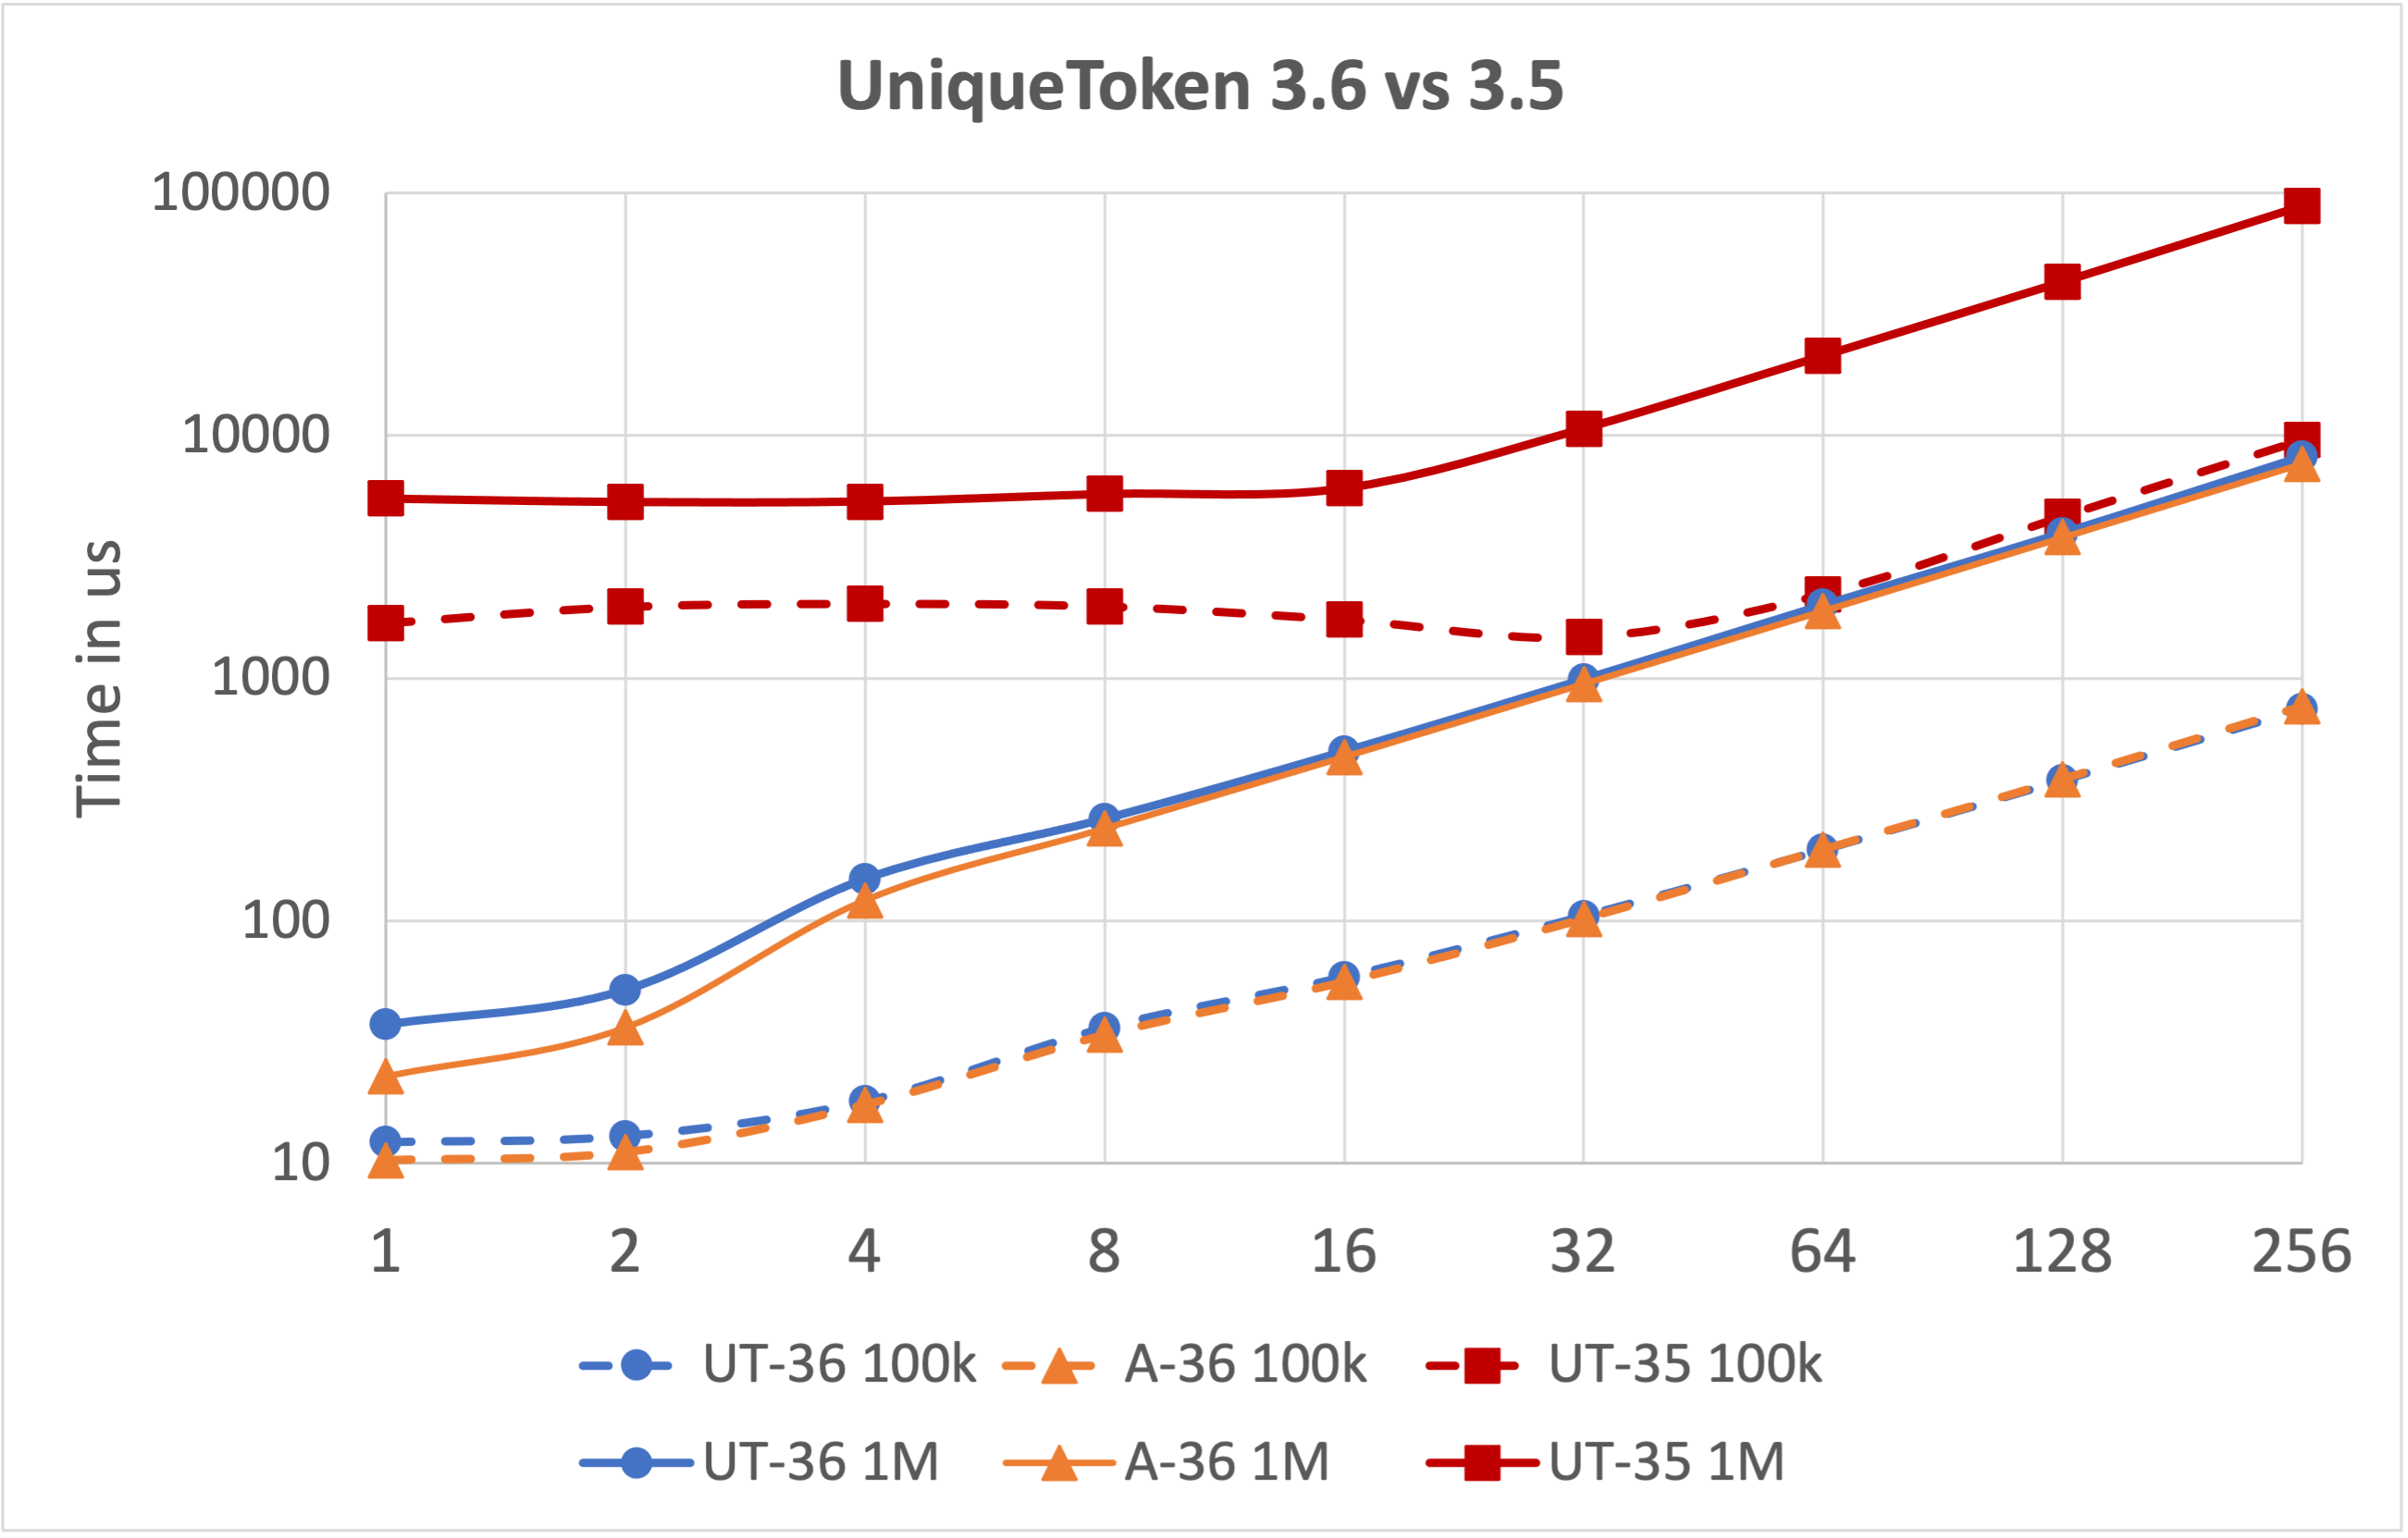
\includegraphics[scale=0.47]{UniqueToken}
\end{center}
\end{frame}


\begin{frame}[fragile]{More Information}

\textbf{Reason for Performance Issue}
\begin{itemize}
  \item Unnecessary many conflicts in acquiring token.
  \item Indicies acquired by threads in the same warp tended to be far apart $->$ results in bad memory access pattern.
\end{itemize}

\vspace{10pt}
\begin{center}
\texttt{UniqueToken} is discussed in the Kokkos Lectures Module 4!

\vspace{20pt}
Remember: still in \texttt{Experimental} namespace.

Feedback is welcome!
\end{center}
\end{frame}


%==========================================================================

\begin{frame}[fragile]

  {\Huge More View Allocation Properties Support}

  \vspace{10pt}

  \textbf{Content:}
  Support \texttt{WithoutInitializing} for
  \begin{itemize}
    \item \texttt{resize}
    \item \texttt{realloc}
    \item \texttt{create\_mirror}
    \item \texttt{create\_mirror\_view}
  \end{itemize}

  \vspace{-20pt}

\end{frame}

%==========================================================================

\begin{frame}{View Allocation Properties}
  Often initialization is not required when allocating.\\~\newline
  New overloads for \texttt{resize}/\texttt{realloc} and \texttt{create\_mirror[\_view]} supported for \texttt{View}-like types
\begin{itemize}
  \item \texttt{DualView}
  \item \texttt{DynamicView}
  \item \texttt{DynRankView}
  \item \texttt{OffsetView}
  \item \texttt{ScatterView}
  \item \texttt{View}
\end{itemize}
\end{frame}

%==========================================================================

\begin{frame}[fragile]{\texttt{Kokkos::resize}}
\begin{code}
template <class I, class T, class... P>
void
resize(const I& arg_prop, View<T, P...>& v,
       const size_t n0, const size_t n1, const size_t n2,
       const size_t n3, const size_t n4, const size_t n5,
       const size_t n6, const size_t n7);

template <class I, class T, class... P>
void
resize(const I& arg_prop, View<T, P...>& v,
       const typename View<T, P...>::array_layout& layout);
\end{code}
\vspace{10pt}

Resizes \texttt{v} to have the new dimensions while preserving the contents for the common subview of the old and new \texttt{View}. The new \texttt{View} is constructed using the View constructor property \texttt{arg\_prop}, e.g., \texttt{WithoutInitializing}.
\end{frame}

%==========================================================================

\begin{frame}[fragile]{\texttt{Kokkos::realloc}}
\begin{code}
template <class I, class T, class... P>
void
realloc(const I& arg_prop, View<T, P...>& v,
        const size_t n0, const size_t n1, const size_t n2,
        const size_t n3, const size_t n4, const size_t n5,
        const size_t n6, const size_t n7);

template <class I, class T, class... P>
void
realloc(const I& arg_prop, View<T, P...>& v,
        const typename View<T, P...>::array_layout& layout);
\end{code}
\vspace{10pt}

Resizes \texttt{v} to have the new dimensions while preserving the contents for the common subview of the old and new \texttt{View}. The new \texttt{View} is constructed using the View constructor property \texttt{arg\_prop}, e.g., \texttt{WithoutInitializing}.
\end{frame}

%==========================================================================

\begin{frame}[fragile]{\texttt{Kokkos::create\_mirror}}
\begin{code}
template <class ViewType>
typename ViewType::HostMirror 
create_mirror(decltype(WithoutInitializing),
              ViewType const& src);

template <class Space, class ViewType>
ImplMirrorType 
create_mirror(decltype(WithoutInitializing),
              Space const& space, ViewType const&);
\end{code}
\vspace{10pt}

Creates a new host accessible \texttt{View} with the same layout and padding as \texttt{src}. The new \texttt{View} will have uninitialized data.
\end{frame}

%==========================================================================

\begin{frame}[fragile]{\texttt{Kokkos::create\_mirror\_view}}
\begin{code}
template <class ViewType>
typename ViewType::HostMirror
create_mirror_view(decltype(WithoutInitializing),
                   ViewType const&);

template <class Space, class ViewType>
ImplMirrorType
create_mirror_view(decltype(WithoutInitializing),
                   Space const& space, ViewType const&);
\end{code}
\vspace{10pt}

If \texttt{src} is not host-accessible, it creates a new host-accessible \texttt{View} with the same layout and padding as \texttt{src}. The new \texttt{View} will have uninitialized data.
Otherwise returns \texttt{src}.
\end{frame}

%==========================================================================

\begin{frame}{Section Summary}
  \begin{itemize}
    \item This release:\\ \texttt{WithoutInitializing} support for \texttt{resize}/\texttt{realloc} and \texttt{create\_mirror[\_view]} for \texttt{View}-like types
    \item Upcoming release: \\Overloads taking \texttt{Kokkos::view\_alloc} unifying the interfaces and allow, e.g., passing execution spaces.
  \end{itemize}
\end{frame}


%==========================================================================

\begin{frame}[fragile]

  {\Huge C++ Standard Algorithms}

  \vspace{10pt}

  {\large Kokkos implementation of a (growing set) of std algorithms}

  \vspace{20pt}

  \textbf{Objectives:}
  \begin{itemize}
  \item {Kokkos iterators}
  \item {Overview of supported algorithms}
  \item {Differences between the Kokkos and std API}
  \item {Examples}
  \item {Summary}
  \end{itemize}

  \vspace{-20pt}

\end{frame}

%==========================================================================

\begin{frame}[fragile]

  \begin{itemize}
  \item Iterators and std algorithms:
    \begin{itemize}
    \item Released with {\bf Kokkos 3.6}
    \item Include via header: \texttt{Kokkos\_StdAlgorithms.hpp}
    \end{itemize}
    \vspace{10pt}

  \item Inside the \texttt{Kokkos::Experimental}
    \begin{itemize}
    \item Please use them and send us feedback!
    \end{itemize}

    \vspace{10pt}
  \item Documentation is available in the Kokkos wiki:\\
    \url{https://github.com/kokkos/kokkos/wiki}

  \end{itemize}

\end{frame}

%==========================================================================

\begin{frame}[fragile]{Kokkos random-access iterators}

\textbf{\texttt{Kokkos::Experimental::\{begin, cbegin, end, cend\}}}

\vspace{10pt}
Declaration:
\begin{code}
template <class DataType, class... Properties>
KOKKOS_INLINE_FUNCTION
auto begin(const Kokkos::View<DataType, Properties...>& view);
\end{code}

\pause
\begin{itemize}
\item \texttt{view}: must be rank-1 with \texttt{LayoutLeft}, \texttt{LayoutRight},
  or \texttt{LayoutStride}.
\item Dereferencing iterators must be done in an execution space where `view` is accessible.
\end{itemize}

\pause
\vspace{5pt}
\texttt{Kokkos::Experimental::distance(first, last);}\\
\texttt{Kokkos::Experimental::iter\_swap(it1, it2);}

\end{frame}
%==========================================================================

\begin{frame}[fragile]{Algorithms: we use categories as in the C++ std}
  \begin{figure}
    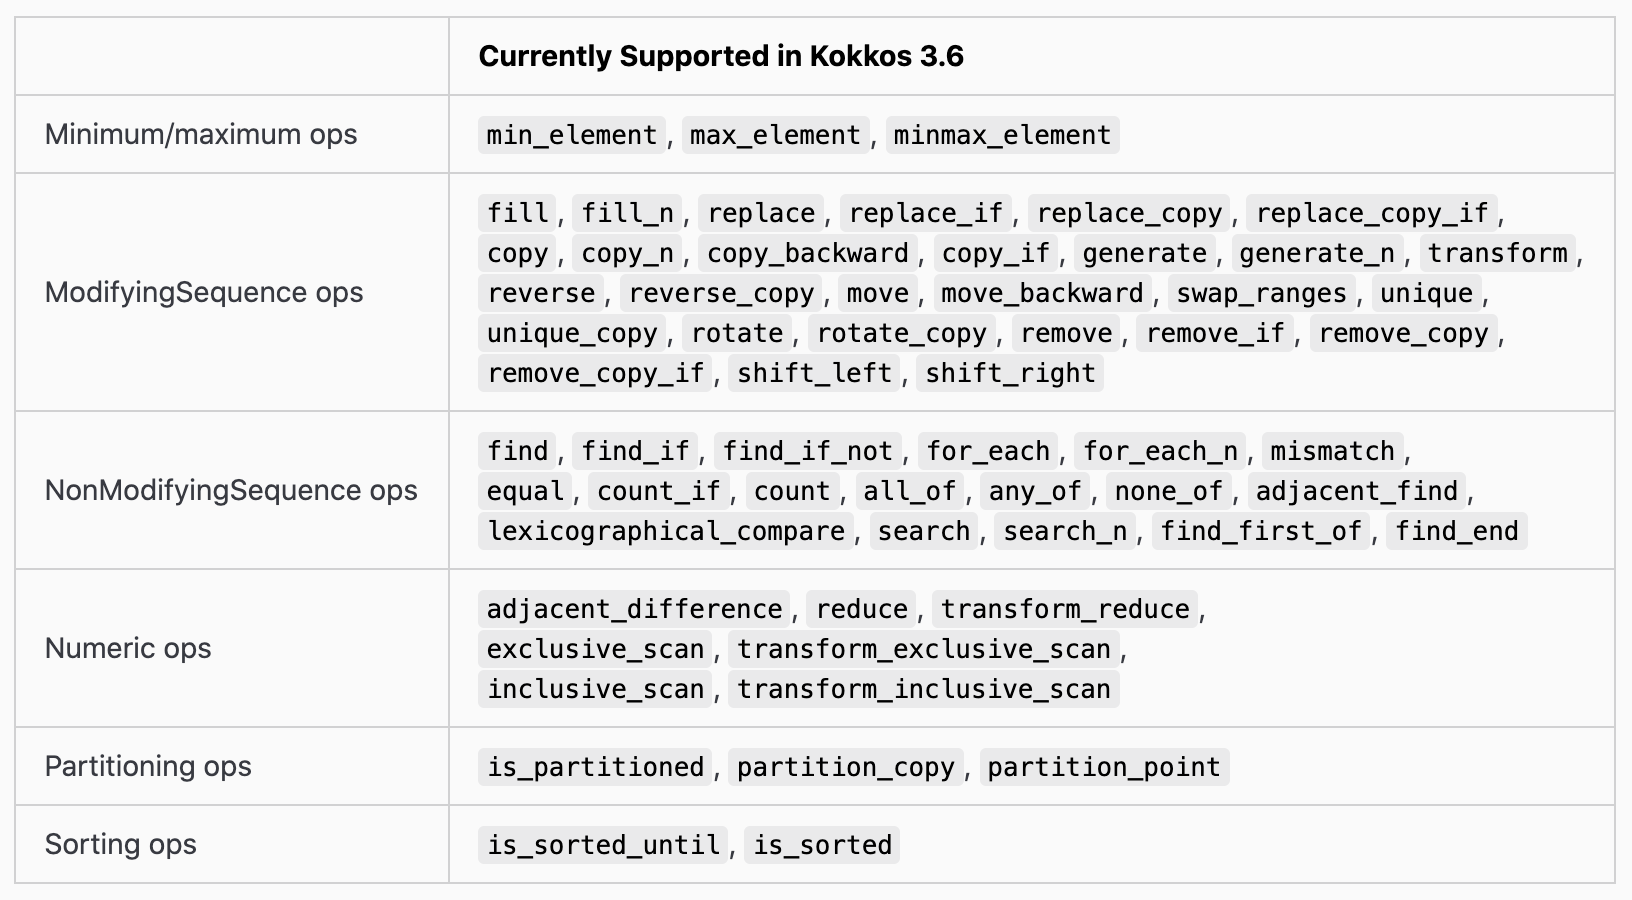
\includegraphics[width=1\linewidth]{algotable.png}
  \end{figure}

\end{frame}
%==========================================================================

\begin{frame}[fragile]{Algorithms: the key difference of our API}

- API accepting iterators:
\begin{code}
template <class ExeSpace, ...>
<return_type> algo_name(const ExeSpace& exespace, <iterators>);

template <class ExeSpace, ...>
<return_type> algo_name(const std::string& label,
                        const ExeSpace& exespace, <iterators>);
\end{code}

\vspace{10pt}
- API accepting Kokkos rank-1 views:
\begin{code}
template <class ExeSpace, ...>
<return_type> algo_name(const ExeSpace& exespace, <views>);

template <class ExeSpace, ...>
<return_type> algo_name(const std::string& label,
                        const ExeSpace& exespace, <views>);
\end{code}
\end{frame}
%==========================================================================

\begin{frame}[fragile]{Algorithms: the API details}

\begin{code}
template <class ExeSpace, ...>
<return_type> algo_name(const ExeSpace& exespace,   (1)
                        <iterators_or_views>);

template <class ExeSpace, ...>
<return_type> algo_name(const std::string& label,   (2)
                        const ExeSpace& exespace,
                        <iterators_or_views>);
\end{code}

\begin{itemize}
\item \texttt{exespace}: iterators/views MUST be accessible from it

\item \texttt{label}: passed to the implementation kernels for debugging
  \begin{itemize}
    \item For (1): ``Kokkos::algo\_name\_iterator\_api\_default'' or \\ \hspace{1.3cm}``Kokkos::algo\_name\_view\_api\_default''
  \end{itemize}

\item iterators: must be {\bf random access iterators}, preferably use \texttt{Kokkos::Experimental::begin,end,cbegin,cend}

\item views: rank-1, \texttt{LayoutLeft, LayoutRight, LayoutStride}
\end{itemize}

\end{frame}
%==========================================================================

\begin{frame}[fragile]{Algorithms: basic example}

  \hspace{-40pt}
  \begin{code}
    int main(){
      // ...
      namespace KE = Kokkos::Experimental;

      Kokkos::View<double*, Kokkos::HostSpace> myView("myView", 13);
      // assuming myView is filled somehow

      const double oldVal{2}, newVal{34};

      // act on the entire view
      KE::replace(Kokkos::DefaultHostExecutionSpace(),
                  KE::begin(myView), KE::end(myView), oldVal, newVal);

      // act on just a subset
      auto startAt = KE::begin(myView) + 4;
      auto endAt   = KE::begin(myView) + 10;
      KE::replace(Kokkos::DefaultHostExecutionSpace(), 
                  startAt, endAt, oldVal, newVal);

      // set label and execution space (assumed enabled)
      KE::replace("mylabel", Kokkos::OpenMP(),
                  myView, oldVal, newVal);
   }
  \end{code}
\end{frame}
%==========================================================================

\begin{frame}[fragile]{Algorithms: example with custom functor for comparison}

  \hspace{-40pt}
  \begin{code} %[basicstyle=\tiny]

     template <class ValueType1, class ValueType2 = ValueType1>
     struct CustomLessThanComparator {
       KOKKOS_INLINE_FUNCTION
       bool operator()(const ValueType1& a, const ValueType2& b) const
       {
        // here we use < but you can put any custom logic needed
        return a < b;
       }
     };

     int main(){
       // ...
       namespace KE = Kokkos::Experimental;
       Kokkos::View<double*, Kokkos::CudaSpace> myView("myView", 13);
       // fill a somehow
       auto res = KE::min_element(Kokkos::Cuda(), myView,
                                  CustomLessThanComparator<double>());
       //...
     }
  \end{code}
\end{frame}
%==========================================================================


\begin{frame}[fragile]{Algorithms: general considerations}

\begin{itemize}
\item Implementations rely on Kokkos parallel for, reduce or scan.

\vspace{10pt}
\item Debug mode enables several checks, e.g.: whether iterators
  identify a valid range, the execution space accessibility, etc.,
  and error messages printed.

\vspace{10pt}
\item If needed, algorithms fence directly the execution space instance provided:
  \hspace{-40pt}
  \begin{code}
    template <class ExeSpace, ...>
    <return_type> algo_name(const ExeSpace& exespace, ...)
    {
      // implementation
      exespace.fence(/*string depends on algorithm*/);
    }
  \end{code}
\end{itemize}

\end{frame}
%==========================================================================

\begin{frame}{Section Summary}

  \begin{minipage}{0.6\textwidth}
    \begin{itemize}
    \item Starting with Kokkos 3.6, Kokkos offers many std algorithms
      %\texttt{minimum/maximum, Numeric, ModifyingSequence, NonModifyingSequence, Partitioning, Sorting} ops
    \item Two main APIs: one for iterators and one for rank-1 views
    \item Checkout the documentation in the Kokkos wiki
    \end{itemize}
  \end{minipage}
  \begin{minipage}{0.38\textwidth}
    \begin{figure}
      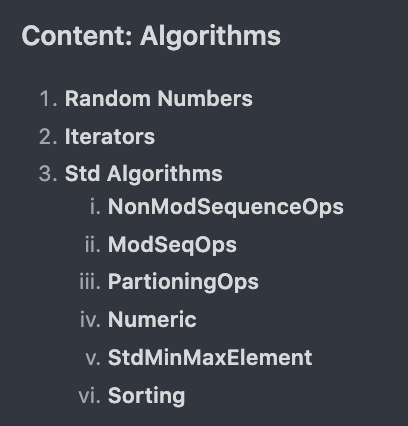
\includegraphics[width=0.7\linewidth]{algowiki.png}
      \caption{Wiki documentation}
    \end{figure}
  \end{minipage}

  \begin{itemize}
  \item{Useful to make your code more expressive, allowing us to worry about having performant implementations}
  \item{Please use them, and let us know of any issues!}
  \item{Try them with the new feature: \texttt{Kokkos::Experimental::partition\_space}}
  \item{In progress: team-level implementations}
  \end{itemize}

\end{frame}


%==========================================================================

\begin{frame}[fragile]

  {\Huge Numerics}

  \vspace{10pt}

  \textbf{Content:}
  \begin{itemize}
    \item {Common mathematical functions}
    \item {Mathematical constants}
    \item {Numeric traits}
  \end{itemize}

  \vspace{-20pt}

\end{frame}

%==========================================================================

\begin{frame}[fragile]{Common math functions}

\textbf{Improvement/Bug fix}

Unconditionally define \texttt{long double} overloads on the host side

\begin{code}
namespace Kokkos::Experimental {
KOKKOS_FUNCTION float       sqrt ( float x );
KOKKOS_FUNCTION float       sqrtf( float x );
KOKKOS_FUNCTION double      sqrt ( double x );
                long double sqrt ( long double x ); // 3.6
                long double sqrtl( long double x ); // 3.6
KOKKOS_FUNCTION double      sqrt ( IntegralType x );
}
\end{code}

\vspace{10pt}

\textbf{Looking ahead}

Math functions promoted to the \texttt{Kokkos::} namespace in 3.7

\end{frame}

%==========================================================================

\begin{frame}[fragile]{Mathematical constants}

\begin{itemize}
  \item{Defined in header \texttt{<Kokkos\_MathematicalConstants.hpp>} which is included from \texttt{<Kokkos\_Core.hpp>}}
  \item{Provides all mathematical constants from \texttt{<numbers>} (since C++20), such as \texttt{pi} and \texttt{sqrt2}}
  \item{All constants are defined  in the \texttt{Kokkos::Experimental::} namespace since Kokkos 3.6}
\end{itemize}

\end{frame}

%==========================================================================

\begin{frame}[fragile]{Numeric traits}

\textbf{Improvement/Bug fix}

\begin{itemize}
  \item{Add missing traits \texttt{denorm\_min}, \texttt{reciprocal\_overflow\_threshold}, and \texttt{\{quiet,silent\}\_NaN}}
  \item{Instantiate numeric traits on cv-qualified types}
\end{itemize}

\end{frame}

%==========================================================================

\begin{frame}{Section Summary}

  \begin{itemize}
    \item{Consistent and portable overload set for standard C library mathematical functions, such as \texttt{fabs}, \texttt{sqrt}, and \texttt{sin}}
    \item{Backport of the C++20 standard library header \texttt{<numbers>} and provides several mathematical constants, such as \texttt{pi} or \texttt{sqrt2}}
    \item{New facility that is being added to the C++23 standard library and is intended as a replacement for \texttt{std::numeric\_limits}}
  \end{itemize}

\end{frame}


%==========================================================================

\begin{frame}[fragile]

        {\Huge \texttt{KOKKOS\_IF\_ON\_\{HOST,DEVICE\}} macros}

  \vspace{-20pt}

\end{frame}

%==========================================================================

\begin{frame}[fragile]{\texttt{\#ifdef \_\_CUDA\_ARCH\_\_} idiom not portable}
\textbf{Motivating example}
\begin{code}[keywords={__CUDA_ARCH__}]
__host__ __device__ void terminate() {
#ifdef __CUDA_ARCH__
  asm("trap;");  // inline PTX assembly when called on device
#else
  _exit();       // OS call when called on the host
#endif
}
\end{code}

\begin{itemize}
\item NVIDIA HPC compiler uses a unified heterogeneous compilation model (single-pass)
\item NVC++ cannot support {\color{blue}\texttt{\_\_CUDA\_ARCH\_\_}} because that assumes split compilation
\end{itemize}

\end{frame}

%==========================================================================

\begin{frame}[fragile]{Use cases}
\textbf{Overloading based on \texttt{\_\_host\_\_ and \_\_device\_\_} attributes}
\begin{code}[keywords={__CUDA_ARCH__}]
struct MyS { int i; };
#ifdef __NVCC__
  #ifndef __CUDA_ARCH__
    __host__ MyS MakeStruct() { return MyS{0};}
  #else
    __device__ MyS MakeStruct() { return MyS{1};}
  #endif
#else
    __host__ MyS MakeStruct() { return MyS{0};}
    __device__ MyS MakeStruct() { return MyS{1};}
#endif
\end{code}

\vspace{10pt}
\textbf{Different class on host/device (NOT SUPPORTED)}
\begin{code}[keywords={__CUDA_ARCH__}]
struct solver {
  // ...
  #ifndef __CUDA_ARCH__
  std::ofstream output_;
  #endif
};
\end{code}

\end{frame}

%==========================================================================

\begin{frame}[fragile]{\texttt{KOKKOS\_IF\_ON\_\{HOST,DEVICE\}} macros}
\textbf{Revisit overloading on host and device example}
\begin{code}[keywords={KOKKOS_IF_ON_HOST,KOKKOS_IF_ON_DEVICE}]
struct MyS { int i; };
KOKKOS_FUNCTION MyS MakeStruct() {
  KOKKOS_IF_ON_HOST(( return MyS{0}; ))
  KOKKOS_IF_ON_DEVICE(( return MyS{1}; ))
}
\end{code}

\textbf{Things to note}
\begin{itemize}
\item Both macros introduce a new scope
\begin{code}[keywords={KOKKOS_IF_ON_HOST}]
  KOKKOS_IF_ON_HOST((
    int x = 0;
    std::cout << x << '\n';
  )) // scope of 'x' ends here
\end{code}
\item Cannot be used in a context that requires constant expressions (\texttt{constexpr})
\item Do not play nice with other preprocessor directives
\end{itemize}

\end{frame}

%==========================================================================

\begin{frame}[fragile]{Preprocessor directives}

\begin{code}[keywords={KOKKOS_IF_ON_HOST,KOKKOS_IF_ON_DEVICE}]

KOKKOS_FUNCTION void host_compute() {
#if KOKKOS_VERSION >= 30700
  auto sqrt2f = Kokkos::sqrtf(2);
  // ...
#else
  auto sqrt2f = 1.41421356237f;
  // ...
#endif
}

KOKKOS_FUNCTION void device_compute() { /* ... */ }

KOKKOS_FUNCTION decltype(auto) compute() {
  KOKKOS_IF_ON_HOST(( return host_compute(); ))
  KOKKOS_IF_ON_DEVICE(( return device_compute(); ))
}
\end{code}

\end{frame}

%==========================================================================

\begin{frame}{Section Summary}

  \begin{itemize}
    \item{{\color{blue}\texttt{\#ifdef \_\_CUDA\_ARCH\_\_}} idiom is not portable}
    \item{Release 3.6 introduces two macros: {\color{blue}\texttt{KOKKOS\_IF\_ON\_HOST}} and {\color{blue}\texttt{KOKKOS\_IF\_ON\_DEVICE}}}
    \begin{alertblock}{Warning!}
       Avoid using as much possible.  These macros are a last resort facility for differentiating between host and device inside a kernel.
       Consider other approaches such as partial template specialization on execution spaces.
    \end{alertblock}
    \item{Upcoming support for NVC++ (in the next release or two)}
  \end{itemize}

\end{frame}

\begin{frame}[fragile]
  {\Huge Kernels update}

  \begin{itemize}
  \item Architectures support
  \item Batched linear solvers
  \item Block Sparse Matrices
  \item Batched GEMM
  \item Mixed precision
  \end{itemize}

\end{frame}

\begin{frame}[fragile]{Platforms/Architecture support (Brian, Luc)}
Architecture support:
\begin{itemize}
  \item Nvidia fully supported with Cuda backend
  \item AMD fully supported with HIP backend, still optimizing for performance
  \item Intel initial support with SYCL backend, more testing and performance optimization needed
\end{itemize}
Spack updated with release 3.6.0, build tested on Summit, Spock/Crusher and initial support on Arcticus.\\
Starting to support streams on device, inquire for details.
\end{frame}

\begin{frame}[fragile]{Batched Linear Solvers (Kim)}
New batched linear solvers are introduced
\begin{itemize}
  \item LU with static pivoting
  \item PCG
  \item GMRES
\end{itemize}
\begin{center}
  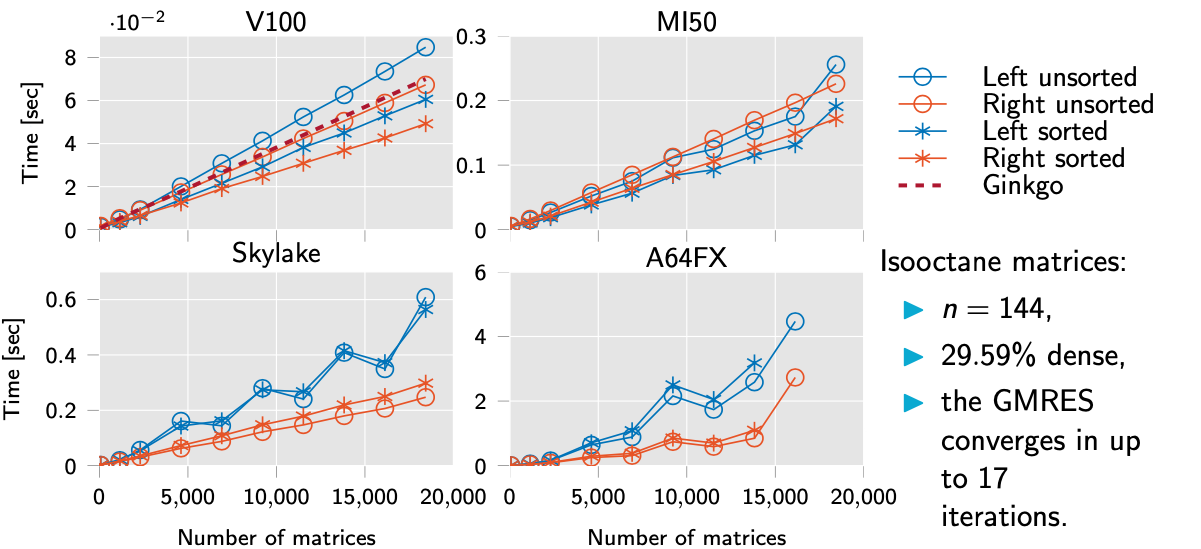
\includegraphics[scale=0.2]{batchedGMRES}
\end{center}
\end{frame}

\begin{frame}[fragile]{Block Sparse Matrices: BsrMatrix (NGA, Luc)}

New BsrMatrix matrix format implemented, supports constant block size sparse matrix mostly geared toward multi-physics systems representation.\\
Currently supported algorithms:
\begin{itemize}
  \item BrsMatrix
  \item Matrix-Vector product using SpMV interface
  \item Matrix-Matrix product using SpGEMM interface
  \item Gauss-Seidel smoother
\end{itemize}
The new format requires less memory and exposes dense linear algebra usage within sparse linear algebra kernels, leading to increased performance compared to point CrsMatrix.

\end{frame}

\begin{frame}[fragile]{Batched GEMM improvements (Evan, Vinh)}
New heuristics and improved interface included a unified interface for all levels of parallelism (TeamVector, Team and Serial) for simplicity.\vspace{-1em}
\begin{columns}[t,onlytextwidth]
  \column{.6\textwidth}
  \begin{itemize}
  \item row-major speedup is 1.17x
  \item column-major speedup is 1.26x
  \item dimensions 2 to 24: single parallel-for with a RangePolicy over entries of C
  \item dimensions $>$ 24: double buffering algorithm based on Magma’s BatchedGemm, Kokkos team cooperatively works on a tile.
  \end{itemize}
  \column{.05\textwidth}
  \column{.35\textwidth}
  \begin{figure}
    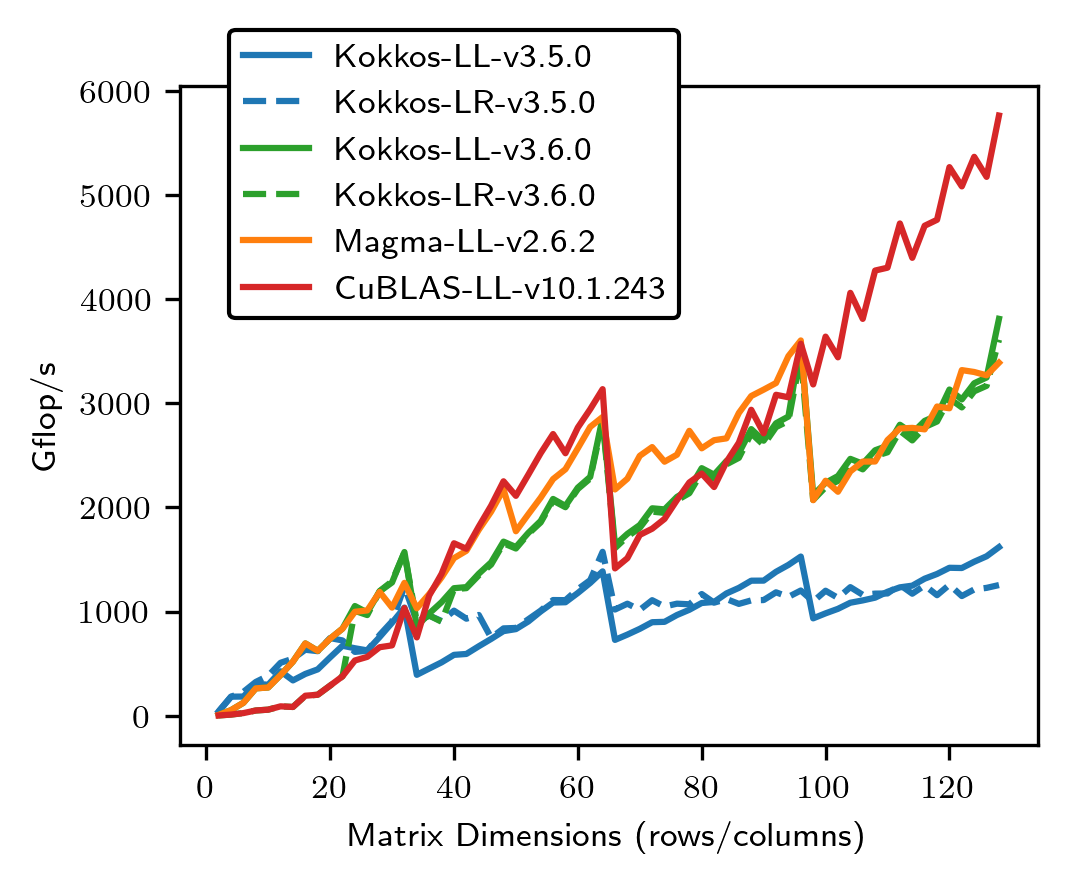
\includegraphics[scale=0.5]{batchedGEMM}
    % \caption{Kokkos BatchedGemm square heuristic, Magma v2.6.2 and CuBlas BatchedGemm on V100 compiled with gcc v8.3.0 and cuda 10.1.243 on V100.}
  \end{figure}
\end{columns}\vspace{1em}
Future work includes additional optimizations to the Kokkos BatchedGemm algorithm.
\end{frame}

\begin{frame}[fragile]{Mixed precision algorithms (Jennifer)}
\begin{columns}[t,onlytextwidth]
  \column{0.475\textwidth}
  \begin{itemize}
  \item Kokkos Kernels provides mixed precisions linear algebra kernels.
  \item GMRES with iterative refinement runs in single precision, residual achieves double precision via iterative refinement
  \item Kokkos Kernels is also providing interfaces for experiments with 16-bit precisions
  \end{itemize}
  \column{0.05\textwidth}
  \column{0.475\textwidth}
  \begin{center}
    \begin{figure}
      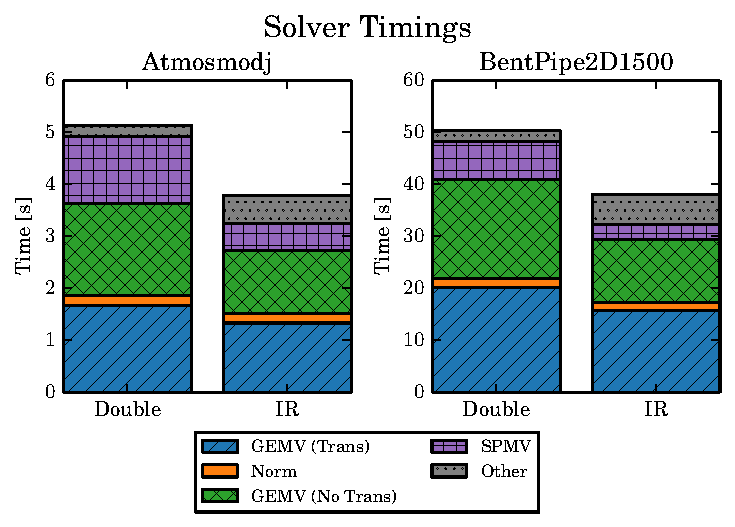
\includegraphics[scale=0.4]{mixed_precision}
      \caption{\tiny Solve times for GMRES(50) double (left) and IR (right) for the matrices Atmosmodj and BentPipe2D1500. Each bar represents total solve time, split up to give a breakdown of time spent in different kernels.}
    \end{figure}
  \end{center}
\end{columns}
\end{frame}

\begin{frame}[fragile]{Collaborations}
Multiple new and ongoing collaborations are cultivated
\begin{itemize}
  \item Nvidia: LU factorization for dense systems
  \item Ginkgo: development of batched gmres
  \item PETSc: providing a portable algebra layer
  \item ExaWind: preconditioner techniques
  \item AMD: library optimization and MFMA usage
  \item ANL: porting and testing on Intel platform
  \item NASA: performance optimization of sparse matrix-vector product
\end{itemize}
and probably many more that I forget...
\end{frame}

\begin{frame}[fragile]{Future focus}
Focus of future work
\begin{itemize}
  \item Performance optimization in Block Sparse algorithms
  \item Format conversion of sparse matrix: Csc2Csr, Coo2Csr
  \item Sparse ILU and TRSV performance improvements
  \item more batched solver features and new batched ODE solvers
  \item more stream support for BLAS and Sparse kernels
  \item fast iterative ILUt algorithm
\end{itemize}
\end{frame}


\end{document}

